\chapter{Πειράματα και Αποτελέσματα}

Στο κεφάλαιο αυτό θα αναλύσουμε τα πειράματα που έγιναν για την εκπαίδευση του μοντέλου παραγωγής κώδικα και θα εξετάσουμε την ποιότητα του παραγώμενου κώδικα.
Θα εξετάσουμε ξεχωριστά κάθε σετ δεδομένων και θα συγκρίνουμε τις επιλογές και τις επιδόσεις των 2 προσεγγίσεων σε καθ' ένα απο αυτά.

\section{Πειράματα εκπαίδευσης}

Ένα πολύ σημαντικό κομμάτι της εκπαίδευσης ενός τέτοιου συστήματος είναι η κατάλληλη επιλογή των υπερπαραμέτρων.
Αποδεικνύεται πως η αποδοτικότερη μέθοδος για την επιλογή τους είναι η τυχαία μέθοδος \cite{Bergstra2012}.
Η υπολογιστική πολυπλοκότητα που εισάγουν τα αναδραστικά νευρωνικά δίκτυα και οι περιορισμένοι υπολογιστικοί πόροι που έχουμε στη διάθεση μας κάνουν αυτή την επιλογή αδύνατη.
Αντ' αυτού επιλέγουμε εμπειρικά τις υπερπαραμέτρους (με δοκιμές) και με οδηγό της επιλογές στη σύγχρονη σχετική βιβλιογραφία.

\subsection{\en{Top 100 Github Javascript Projects} Πειράματα}

Το σετ δεδομένων αυτό αποτελείται από τα 100 πιο δημοφιλή \en{projects} σε γλώσσα \en{javascript} στον ιστότοπο αποθετηρίων λογισμικού \en{github}.
Μετά το \en{prepocessing} παίρνουμε ακολουθίες συνολικού μήκους περίπου 79 εκατομμυρίων χαρακτήρων.
Υπάρχουν 212 διαφορετικοί χαρακτήρες, συμπεριλαμβανομένων των ειδικών χαρακτήρων αρχής και τέλους αρχείων.
Χρησιμοποιούμε το 95\% των δεδομένων για την εκπαίδευση του συστήματος και το υπόλοιπο 5\% για την επικύρωση της μάθησης.
Η έλλειψη ξεχωριστού τεστ σετ μπορεί να σημαίνει πως τα αποτελέσματα μας κάνουν \en{overfit} στα δεδομένα επικύρωσης, αλλά αυτό είναι δευτερευούσης σημασίας αφού στόχος μας είναι να παράξουμε κώδικα και δεν υπάρχουν διαθέσιμα συγκριτικά αποτελέσματα (\en{benchmark results}) για τον σκοπό αυτό.

Η στρατηγική επιλογής των παραμέτρων έχει ως εξής: Για να είναι οι δύο προσεγγίσεις συγκρίσιμες κρατάμε ίδιο το μέγεθος των κρυφών επιπέδων.
Από αυτή την επιλογή εξαρτάται κυρίως ο αριθμός συνολικών παραμέτρων προς εκπαίδευση.
Για το πρώτο σετ δεδομένων αποφασίζουμε τον αριθμό αυτό σε 1024, αριθμός αρκετά μεγάλος ώστε να είναι αντιμετωπίσιμο από το σύστημα το ογκώδες σετ δεδομένων.

Η επόμενη υπερ-παράμετρος που πρέπει να αποφασιστεί είναι το μήκος της εκπαιδευτικής ακολουθίας, η μεταβλητή $k_2$ του αλγορίθμου \en{TBPTT}.
Η υπερ-παράμετρος αυτή έχει μεγάλη σχέση τόσο με την ποιότητα του παραγώμενου κώδικα, αφού ελέγχει πόσους από τους προηγούμενους χαρακτήρες <<βλέπει>> το σύστημα, αλλά και με τον χρόνο εκτέλεσης μιας εποχής, αφού μεγαλύτερες ακολουθίες εισάγουν υπολογιστική πολυπλοκότητα.
Το μέγεθος των εκπαιδευτικών ακολουθιών αποφασίζεται στους 100 χαρακτήρες και για τα δύο μοντέλα.

Ο ρυθμός εκμάθησης είναι άμεσα συνδεδεμένος με το μέγεθος παρτίδας.
Όσο περισσότερα παραδείγματα βλέπει ταυτόχρονα το σύστημα τόσο πιο σίγουρο θα πρέπει να είναι για τα συμπεράσματα του.
Εξαγωγή δυνατών συμπερασμάτων από λιγοστά παραδείγματα πρέπει να αποφεύγεται.
Επιπρόσθετα υπάρχει και ένας φυσικός περιορισμός στο πόσα παραδείγματα μπορούν να δείχνονται ταυτόχρονα, η μνήμη της επεξεργαστικής μας μονάδας.
Τελικώς δείχνουμε 200 ακολουθίες σε κάθε βήμα εκμάθησης και θέτουμε τον ρυθμό εκμάθησης στην τιμή 0.002, ώστε να γεμίζουμε όσο καλύτερα γίνεται την μνήμη του υπολογιστικού συστήματος αλλά να συνεχίσουμε να μαθαίνουμε αποτελεσματικά.
Σημειώνεται πως η προτεινόμενη τιμή για τον ρυθμό εκμάθησης της \en{rmsprop} είναι το 0.001.

Τέλος, επειδή το σετ δεδομένων αυτό είναι αρκετά ογκώδες και περίπλοκο, είναι δύσκολο το μοντέλο μας να κάνει \en{overfit}. Έτσι, δε χρειάζεται η πιθανότητα dropout να είναι εξαιρετικά μεγάλη.
Επιλέγουμε την υπερ-παράμετρο αυτή στο 20\%, ενώ η γενική προτεινόμενη τιμή είναι 40\% με 50\%.
Ο αριθμός των εποχών αποφασίζεται έτσι ώστε κανένα από τα 2 μοντέλα να μην βελτιώνει τις επιδόσεις του στο σετ δεδομένων επιβεβαίωσης.
Ο αριθμός αυτός προκύπτει στις 60 εποχές.
Στον πίνακα \ref{hyper1} παρουσιάζονται συνοπτικά οι παραπάνω αποφάσεις.

\begin{table}[]
\centering
\caption{Υπερπαράμετοι για τα \en{top 100 Github js projects}}
\begin{tabularx}{\textwidth}{|X|X|X|}
\hline
                    & \en{char-rnn} & \en{labeled-char-rnn} \\
\hline
\en{\#} Παραμέτρων       & 23Μ             & 23Μ                     \\
\hline
\en{\#} Χαρακτήρων       & 212             & 212, 8                  \\
\hline
\en{\#} Εποχών       & 40             & 60                  \\
\hline
Μέγεθος \en{LSTM}  & 1024            & 1024                    \\
\hline
Μήκος Ακολουθίας    & 100             & 100                     \\
\hline
Ρυθμός Εκμάθησης    & 0.002           & 0.002                   \\
\hline
\% \en{Dropout}     & 20              & 20                      \\
\hline
Μέγεθος Παρτίδας    & 200             & 200                     \\
\hline
\end{tabularx}
\label{hyper1}
\end{table}

Η εκπαίδευση έγινε σε μία κάρτα γραφικών \en{Nvidia Gtx 960} με 4 \en{gb RAM}.
Η εκπαίδευση διαρκεί 6 περίπου ημέρες για το πρώτο μοντέλο και 7 περίπου για το δεύτερο.
Όπως αναφέραμε, η παρακολούθηση των επιδόσεων και η επιλογή των σετ βαρών για την παραγωγή κώδικα γίνεται σύμφωνα με την μετρική \en{average cross entropy per minibatch}.
Σημειώνεται πως η σύγκριση των μοντέλων στην μετρική αυτή γίνεται μόνο στο κομμάτι που αφορά την πρόβλεψη χαρακτήρων.
Στην εικόνα \ref{training1} φαίνεται η εξέλιξη της εκπαίδευσης των 2 μοντέλων στην περίοδο 40 και 60 εποχών στο σετ εκπαίδευσης και το σετ επαλήθευσης. 
%TODO Διάγραμμα training me σχόλια περι overfittinh και τετοια και επιλογής μοντέλο και ξαναγραψιμο της μετρικής που χρησιμοποιείται 1 + 0.2. Σχολιασμός των accuracy
Ως μοντέλα παραγωγής, επιλέγουμε αυτά με τα βάρη τις 38ης εποχής για το μοντέλο \en{char-rnn} και της 53ης εποχής για το μοντέλο \en{labeled-char-rnn}, αφού παρουσιάζουν την ελάχιστη τιμή της μετρικής μας.
Οι επιδόσεις των μοντέλων αυτών αντιστοιχούν σε 85.6\% και 87.2\% ποσοστιαία επιτυχία στην πρόβλεψη του επόμενου χαρακτήρα.
Η επιτυχία πρόβλεψης του είδους του χαρακτήρα στο σετ επαλήθευσης βρίσκεται πάνω από το 97\%.
Τα αποτελέσματα της εκπαιδευτικής διαδικασίας είναι σε πρώτη όψη ικανοποιητικά. Οι καμπύλες εκπαίδευσης και επαλήθευσης μένουν σε κοντινά επίπεδα και για τα δύο μοντέλα, γεγονός που μαρτυρά καλή γενίκευση των χαρακτηριστικών που μαθαίνονται. Η ευστοχία, ιδιαίτερα, της ανάθεσης είδους στον επόμενο χαρακτήρα κυμαίνεται σε πολύ υψηλά επίπεδα. 

\begin{figure}[h]
	\caption{Καμπύλες εκμάθησης για τα \en{top 100 github js projects}}
	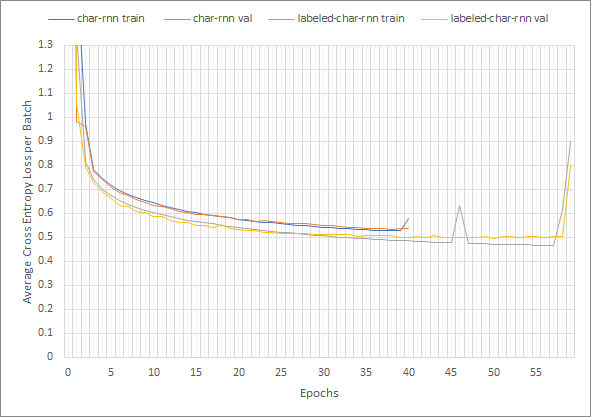
\includegraphics[trim = 2 2 2 2, clip, keepaspectratio]{images/training1.png}
	\centering
	\label{training1}
\end{figure}

\subsection{\en{Top 200 npm Projects} Πειράματα}

Το δεύτερο σετ δεδομένων αποτελείται από τις 200 πιο δημοφιλείς βιβλιοθήκες \en{javascript} του ιστοχώρου \en{www.npmjs.com}.
Οι ακολουθίες μετά την προ-επεξεργασία αριθμούν περίπου 49 εκατομμύρια χαρακτήρες με 210 διαφορετικούς χαρακτήρες. 
Σε αυτό το πείραμα χωρίζουμε το 90\% των ακολουθιών στο σετ εκπαίδευσης και το 10\% στο σετ επαλήθευσης, επειδή έχουμε λιγότερα δεδομένα και θέλουμε να αποφύγουμε μεγάλη διακύμανση στο σετ επαλήθευσης.

Οι αποφάσεις των υπερ-παραμέτρων βασίζονται στις παρατηρήσεις μας από τα προηγούμενα πειράματα. Έτσι, κρατάμε ίδιο το μέγεθος παρτίδας, τον ρυθμό εκμάθησης και το μήκος ακολουθίας.
Το σετ εκπαίδευσης έχει μικρότερο μέγεθος από το προηγούμενο πείραμα και από τις πρώτες δοκιμές παρατηρούμε σημαντικό \en{overfitting}.
Προς την κατεύθυνση καλύτερης γενίκευσης των συμπερασμάτων του συστήματος, αρχικά μικραίνουμε το δίκτυο θέτοντας το μέγεθος \en{LSTM} se 512, κίνηση η οποία μειώνει σημαντικά τις εκπαιδεύσιμες παραμέτρους του συστήματος.
Έπειτα αυξάνουμε την πιθανότητα \en{dropout} σε 30\% και 40\% που αποτέλεσμα έχει την αργότερη εκπαίδευση του αναδραστικού νευρωνικού δικτύου.
Για να αποζημιώσουμε την τελευταία μας επιλογή αυξάνουμε τις εκπαιδευτικές εποχές του μοντέλου σε 60 και 80 αντίστοιχα.
Οι εκπαιδευτικές επιλογές συνοψίζονται στον πίνακα \ref{hyper2}.

\begin{table}[]
\centering
\caption{Υπερπαράμετοι για τα \en{top 200 npm js projects}}
\begin{tabularx}{\textwidth}{|X|X|X|}
\hline
                    & \en{char-rnn} & \en{labeled-char-rnn} \\
\hline
\en{\#} Παραμέτρων       & 10M             & 10M                     \\
\hline
\en{\#} Χαρακτήρων       & 210             & 210, 8                  \\
\hline
\en{\#} Εποχών       & 60             & 80                  \\
\hline
Μέγεθος \en{LSTM}  & 512            & 512                    \\
\hline
Μήκος Ακολουθίας    & 100             & 100                     \\
\hline
Ρυθμός Εκμάθησης    & 0.002           & 0.002                   \\
\hline
\% \en{Dropout}     & 30              & 40                      \\
\hline
Μέγεθος Παρτίδας    & 200             & 200                     \\
\hline
\end{tabularx}
\label{hyper2}
\end{table}

Η διαδικασία που ακολουθείται είναι η ίδια με του προηγούμενου πειράματος, δηλαδή εκπαιδεύουμε το σύστημα σε μία κάρτα γραφικών \en{Nvidia Gtx 960} με 4 \en{gb RAM} και επιλέγουμε το μοντέλο με τις καλύτερες επιδόσεις στη μετρική πρόβλεψης χαρακτήρων.
Η εκπαίδευση του \en{char-rnn} διαρκεί 3 ημέρες ενώ του \en{labeled-char-rnn} διαρκεί περίπου 4. Η εξέλιξη της εκπαίδευσης φαίνεται στην εικόνα \ref{training2}.

\begin{figure}[h]
	\caption{Καμπύλες εκμάθησης για τα \en{top 200 npm js projects}}
	\label{training2}
	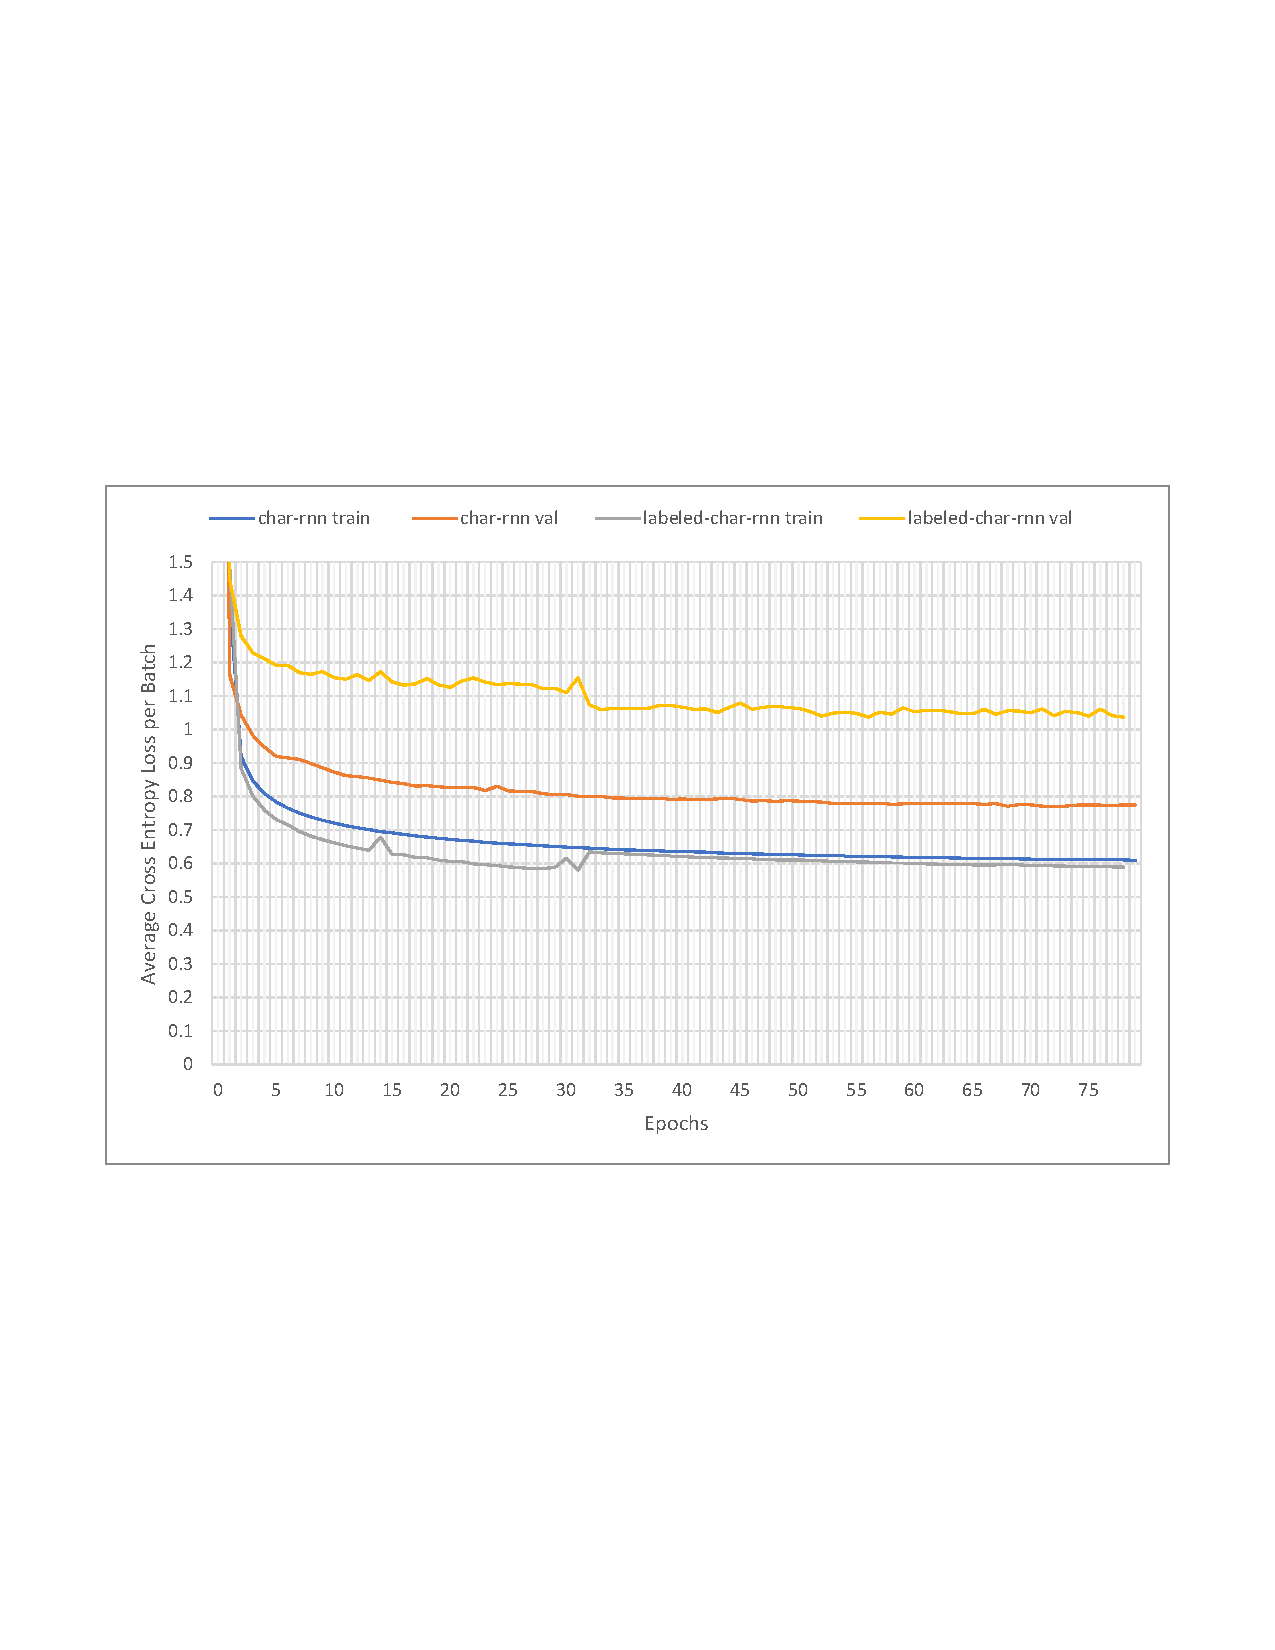
\includegraphics[width=\textwidth, trim = 25 220 25 220, clip, keepaspectratio]{images/training2.pdf}
	\centering
\end{figure}


Το επιλεγόμενο μοντέλο για το \en{char-rnn} είναι αυτό της 72ης εποχής με ποσοστό επιτυχίας πρόβλεψης 78\%. Για το μοντέλο \en{labeled-char-rnn} το επιλεγόμενο μοντέλο είναι αυτό της 78ης εποχής με ποσοστό επιτυχίας 72.3\% την πρόβλεψη χαρακτήρων και 94.7. Είναι εμφανές από το διάγραμμα ότι τα μοντέλα μας δυσκολεύονται περισσότερο να γενικεύσουν τα συμπεράσματα που εξάγουν από αυτό το σετ δεδομένων. Η ικανότητα πρόβλεψης του είδους του επόμενου χαρακτήρα παραμένει σε σχετικά υψηλά επίπεδα αλλά η προσθήκη της δεν βελτιώνει τις επιδόσεις στο σετ επιβεβαίωσης. Θα εξετάσουμε αναλυτικότερα τα αποτελέσματα αυτά στο υποκεφάλαιο των αποτελεσμάτων και στο κεφάλαιο των συμπερασμάτων.

\section{Αποτελέσματα}

Χρησιμοποιούμε τα μοντέλα που εκπαιδεύτηκαν παραπάνω για να παράξουμε 100 αρχεία κώδικα για κάθε προσέγγιση και κάθε ομάδα μοντέλων.
Επιλέγουμε ένα \en{javascript project} με το οποίο αρχικοποιούμε κάθε ομάδα μοντέλων. 
Η αρχικοποίηση του μοντέλου γίνεται με σκοπό την έμμεση οδήγηση του.
Αρχικά θα εξετάσουμε την ποιότητα του κώδικα εποπτικά και έπειτα θα χρησιμοποιήσουμε το εργαλείο \en{jshint} για να κάνουμε στατική ανάλυση του κώδικα.

\subsection{\en{Top 100 Github Javascript Projects} Παραγώμενος κώδικας}

Επιλέγουμε ένα \en{project} που δεν έχει εμφανιστεί στη διάρκεια της εκπαίδευσης και της επαλήθευσης.
Συγκεκριμένα επιλέγουμε το \en{hyper terminal} που είναι το πιο δημοφιλές \en{javascript project} στο \en{github} το πρώτο εξάμηνο του 2017.
Ο κώδικας 5.1 είναι ένα αρχείο από το \en{project} αυτό.

\selectlanguage{english}
\lstinputlisting[language=JavaScript, caption={\tg{Δείγμα κώδικα απο το }\en{hyper terminal}}]{code/hyper.js}
\selectlanguage{greek}

Οι κώδικες 5.2, 5.3 είναι δημιουργήματα των μοντέλων \en{char-rnn} και \en{labeled-char-rnn} αντίστοιχα. Τα αρχεία αυτά επιλέχτηκαν χάρη στο μικρό μέγεθός τους και την συντακτική ορθότητα.

\selectlanguage{english}
\lstinputlisting[language=JavaScript, caption={\tg{Δείγμα κώδικα από το }\en{char-rnn}}]{code/charrnnGithub.js}
\selectlanguage{greek}

Ήδη εποπτικά παρατηρούμε τη δυνατότητα και των δύο μοντέλων να αναπαράγουν συντακτικές δομές, όπως οι παρενθέσεις και οι αγκύλες, αλλά και λογικές, όπως οι συναρτήσεις και οι δομές πολλαπλών επιλογών.
Φαινομενικά αυτό είναι ένα συνηθισμένο αρχείο \en{javascript}.
Με μία δεύτερη, αναλυτικότερη ματιά παρατηρούμε σημαντικά λάθη στη χρήση μη ορισμένων μεταβλητών, την ύπαρξη γραμματικών λαθών και ενέργειες χωρίς αποτέλεσμα. 
Είναι εύκολο να συμπεράνει κανείς, ίσως και χωρίς να είναι γνώστης της γλώσσας, πως τα προγράμματα αυτά δεν θα καταφέρουν να μεταφραστούν. 
Για την καλύτερη εκτίμηση των αποτελεσμάτων των νευρωνικών δικτύων, και για τη σύγκριση των δύο  θα ακολουθήσουμε μια πιο ποσοτική προσέγγιση. 
Με τη χρήση του εργαλείου ανάλυσης κώδικα \en{jshint} θα εξετάσουμε τον αριθμό των συντακτικών και διαφόρων άλλων λαθών \en{(Errors)} που εντοπίζονται και μέχρι πιο σημείο καταφέρνουν να αναγνωστούν πριν βρεθεί ένα ανεπανόρθωτο συντακτικό λάθος (\en{\% Scanned Lines}).
Σημειώνεται πως τα μοντέλα αποφασίζουν αυτόνομα το μήκος του κώδικα, με τη χρήση των ειδικών χαρακτήρων, αλλά τίθεται ένα άνω όριο 15000 χαρακτήρων στο οποίο θεωρούμε ότι το αρχείο ξεφεύγει διαχειρισιμότητας λόγω μεγέθους.
Στις εικόνες \ref{static-github-char} - \ref{MCE2-githubLabeled} φαίνονται τα αποτελέσματα της παραπάνω ανάλυσης και το μήκος των παραγώμενων αρχείων.

\selectlanguage{english}
\lstinputlisting[language=JavaScript, caption={\tg{Δείγμα κώδικα απο το }\en{labeled-char-rnn}}]{code/labeledcharrnnGithub.js}
\selectlanguage{greek}

\begin{figure}[!htb]
	\caption{Στατική ανάλυση κώδικα για τα αποτελέσματα του \en{char-rnn} μοντέλου}
	\label{static-github-char}
	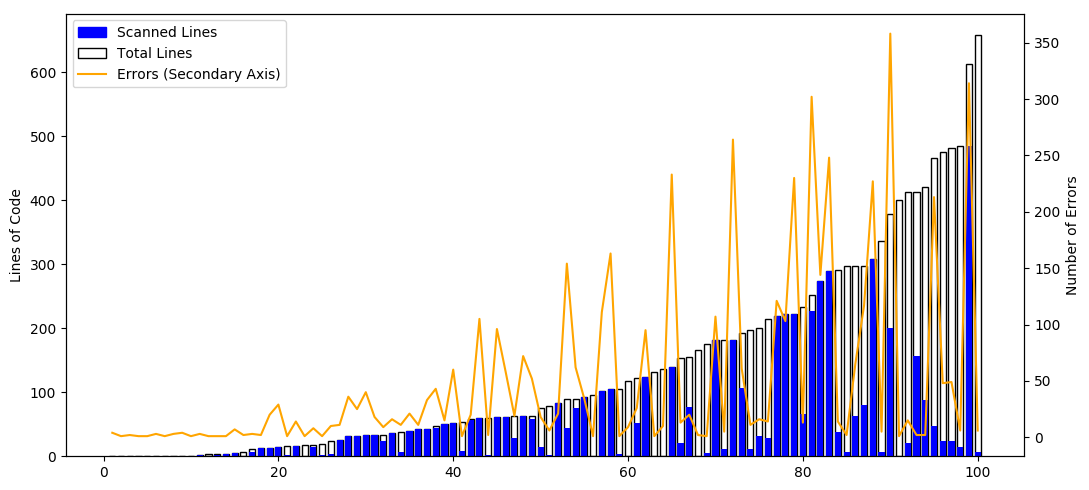
\includegraphics[width=\textwidth, keepaspectratio]{images/jshint-githubChar.png}
\end{figure}

\begin{figure}[!htb]
	\caption{Στατική ανάλυση κώδικα για τα αποτελέσματα του \en{labeled-char-rnn} μοντέλου}
	\label{static-github-labeled}
	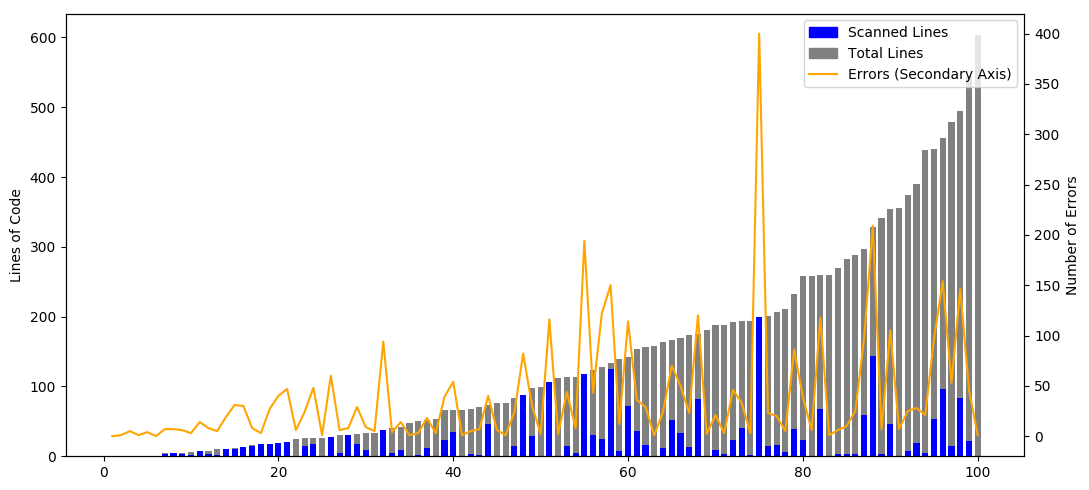
\includegraphics[width=\textwidth, keepaspectratio]{images/jshint-githubLabeled.png}
\end{figure}

\begin{figure}[!htb]
	\caption{Συνηθέστερο λάθος των αρχείων του \en{char-rnn}}
	\label{MCE1-githubchar}
	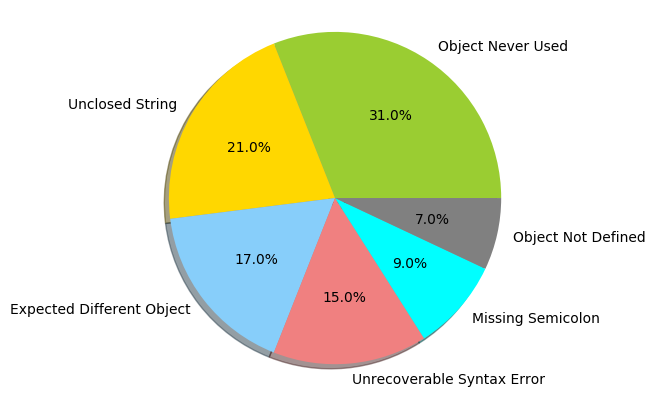
\includegraphics[width=\textwidth, keepaspectratio]{images/MCE-githubchar.png}
\end{figure}

\begin{figure}[!htb]
	\caption{Δεύτερο συνηθέστερο λάθος των αρχείων του \en{char-rnn}}
	\label{MCE2-githubchar}
	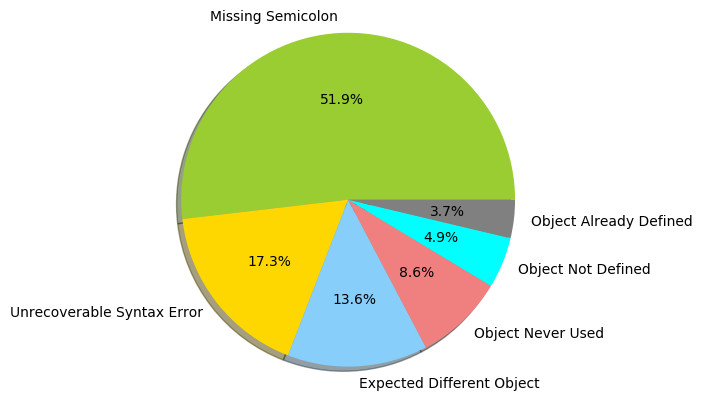
\includegraphics[width=\textwidth, keepaspectratio]{images/MCE2-githubchar.png}
\end{figure}

\begin{figure}[!htb]
	\caption{Συνηθέστερο λάθος των αρχείων του \en{labeled-char-rnn}}
	\label{MCE1-githubLabeled}
	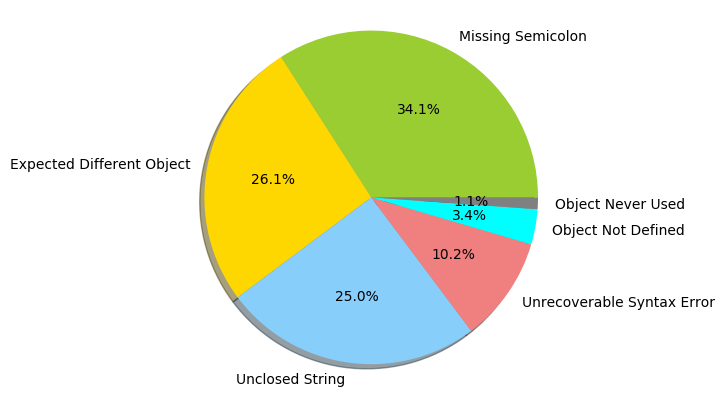
\includegraphics[width=\textwidth, keepaspectratio]{images/MCE-githubLabeled.png}
\end{figure}

\begin{figure}[!htb]
	\caption{Δεύτερο συνηθέστερο λάθος των αρχείων του \en{labeled-char-rnn}}
	\label{MCE2-githubLabeled}
	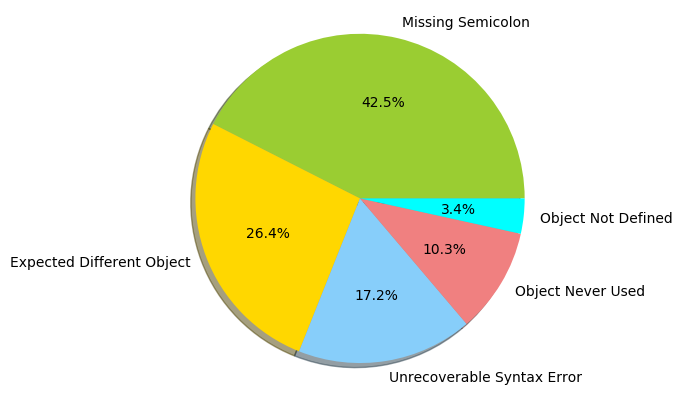
\includegraphics[width=\textwidth, keepaspectratio]{images/MCE2-githubLabeled.png}
\end{figure}

Στα σχήματα \ref{static-github-char} και \ref{static-github-labeled} μπορούμε να συγκρίνουμε τις επιδόσεις των δύο μοντέλων.
Τα στατιστικά των 100 αρχείων εχουν ταξινομηθεί κατά   τον αύξοντα αριθμό γραμμών.
Αρχικά παρατηρούμε πως και τα δύο μοντέλα παράγουν κάποια κενά αρχεία ή αρχεία με 1 ή 2 γραμμές.
Το μέσο μήκος των αρχείων είναι αρκετά κοντινό (137 - 142 γραμμές) και το δεύτερο μοντέλο καταφέρνει να κλείσει τα αρχεία σε λιγότερο από 15000 χαρακτήρες 9\% των φορών ενώ το πρώτο 6\%.
Αν και το δεύτερο μοντέλο έχει περισσότερη πληροφορία για τον κώδικα, παράγει αρχεία που ολοκληρώνουν την ανάλυση κώδικα με αρκετά μικρότερη συχνότητα.
Η γενική εικόνα που παίρνουμε από την ανάλυση αυτή είναι απογοητευτική για το δεύτερο μοντέλο, που ενώ έχει στη διάθεση του περισσότερη πληροφορία αποτυγχάνει να την αποτυπώσει με τρόπο που να παράγει ποιοτικά αποτελέσματα.

Τα είδη των συνηθέστερων λαθών μαρτυρούν τις αδυναμίες της προσέγγισης μας στην παραγωγή κώδικα.
Ακόμα και αν καταφέρνουν να δημιουργηθούν μικρά κομμάτια λειτουργικού κώδικα η έλλειψη ανεξάρτητης μνήμης και η στοχαστική φύση της παραγωγής δυσκολεύουν τα μοντέλα ως προς τη διαχείριση των διαφόρων μεταβλητών, τη χρήση της σύνταξης και τη επίτευξη του τελικού σκοπού.
Αυτή είναι η κύρια αιτία των λαθών \en{'Object Already Defined, Object Not Defined, Object Never Used, Expected Different Object}.
Αρκετά συχνά η δημιουργία αλφαριθμητικών ξεφεύγει της διαχείρισης του μοντέλου και συνεχίζεται να γράφεται κώδικας μέσα σε κάποιο αλφαριθμητικό - που είναι ο κύριος λόγος της ύπαρξης του \en{Unclosed String} σε συνδυασμό με το \en{Missing Semicolon}.

\subsection{\en{Top 200 npm Projects} Παραγώμενος κώδικας}

Ακολουθούμε ανάλυση όμοια με την προηγούμενη υποενότητα.
Το \en{project} αρχικοποίησης που χρησιμοποιείται είναι το \en{lodash}, μια βιβλιοθήκη της \en{javascript} που διευκολύνει τη διαχείριση διανυσμάτων, αντικειμένων, αλφαριθμητικών και τη διαδικασία του \en{unit testing}. Ο κώδικας 5.4 είναι του ιδίου \en{project} και οι κώδικες 5.5, 5.6 είναι επιλεγμένοι κώδικες των παραγώμενων μοντέλων. 
%\pagebreak

\selectlanguage{english}
\lstinputlisting[language=JavaScript, caption={\tg{Δείγμα κώδικα απο το }\en{lodash}}]{code/lodash.js}
\selectlanguage{greek}

\selectlanguage{english}
\lstinputlisting[language=JavaScript, caption={\tg{Δείγμα κώδικα απο το }\en{char-rnn}}]{code/charnpm.js}
\selectlanguage{greek}

\pagebreak

\selectlanguage{english}
\lstinputlisting[language=JavaScript, caption={\tg{Δείγμα κώδικα απο το }\en{labeled-char-rnn}}]{code/npmLabel.js}
\selectlanguage{greek}

Στα σχήματα \ref{static-npm-char} και \ref{static-npm-labeled} μπορούμε να συγκρίνουμε τις επιδόσεις των δύο μοντέλων.
To \en{dataset} αυτό περιέχει κατά μέσο όρο μικρότερα αρχεία οπότε και τα μεγέθη των παραγώμενων αρχείων είναι μικρότερα (113 - 47 γραμμές). 
Και πάλι, το \en{labeled-char-rnn} μοντέλο κλείνει με μεγαλύτερη συνέπεια τα αρχεία του.
Τα ποσοστά ολοκλήρωσης της συντακτικής ανάλυσης και οι μέσοι όροι λαθών δείχνουν βελτίωση σε σχέση με το προηγούμενο σετ δεδομένων, ενώ τα παρόντα μοντέλα χρησιμοποιούν σημαντικά λιγότερες παραμέτρους.
Ωστόσο, και σε αυτό το πείραμα το \en{labeled-char-rnn} μοντέλο αδυνατεί να χρησιμοποιήσει την παραπάνω πληροφορία που του δίνεται. Τα μοτίβα των συνηθισμένων λαθών επαναλαμβάνονται (\ref{MCE1-npmchar} - \ref{MCE2-npmlabeled})

\begin{figure}
	\caption{Στατική ανάλυση κώδικα για τα αποτελέσματα του \en{char-rnn} μοντέλου}
	\label{static-npm-char}
	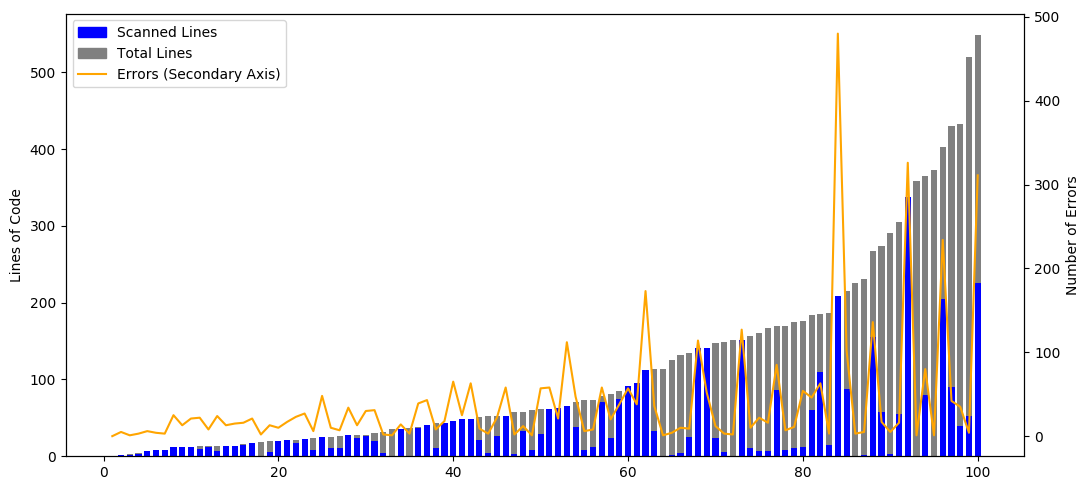
\includegraphics[width=\textwidth, keepaspectratio]{images/jshint-npmchar.png}
\end{figure}

\begin{figure}
	\caption{Στατική ανάλυση κώδικα για τα αποτελέσματα του \en{labeled-char-rnn} μοντέλου}
	\label{static-npm-labeled}
	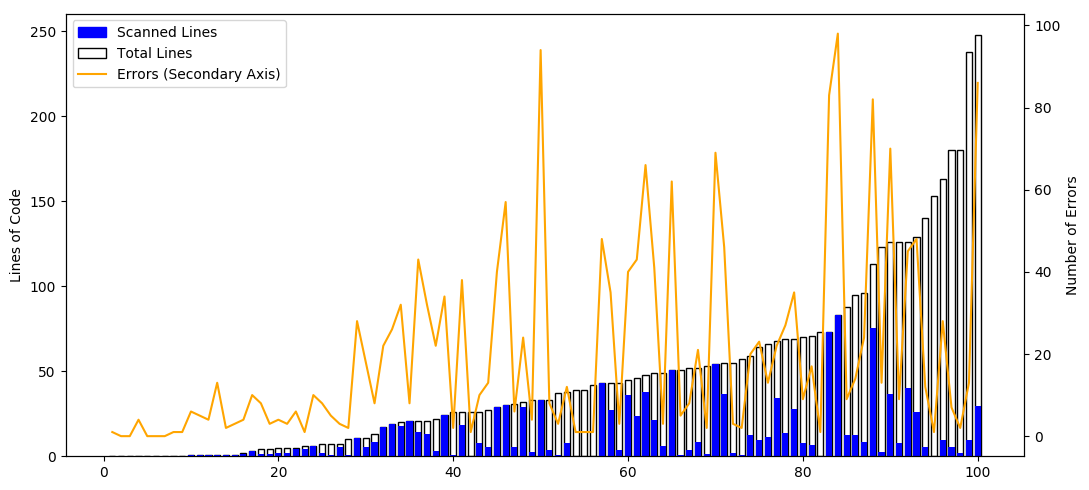
\includegraphics[width=\textwidth, keepaspectratio]{images/jshint-npmlabeled.png}
\end{figure}

\begin{figure}
	\caption{Συνηθέστερο λάθος των αρχείων του \en{char-rnn}}
	\label{MCE1-npmchar}
	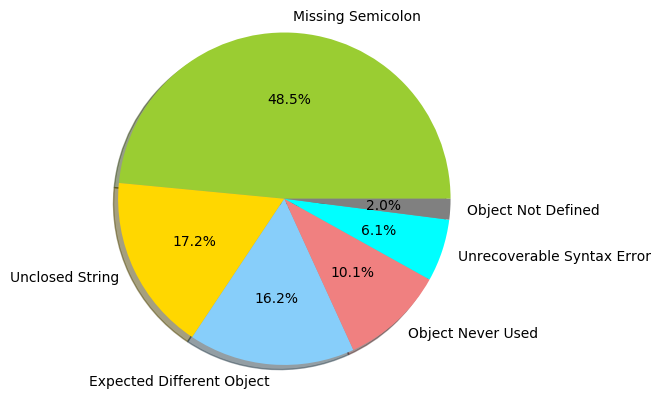
\includegraphics[width=\textwidth, keepaspectratio]{images/MCE-npmchar.png}
\end{figure}

\begin{figure}
	\caption{Δεύτερο συνηθέστερο λάθος των αρχείων του \en{char-rnn}}
	\label{MCE2-npmchar}
	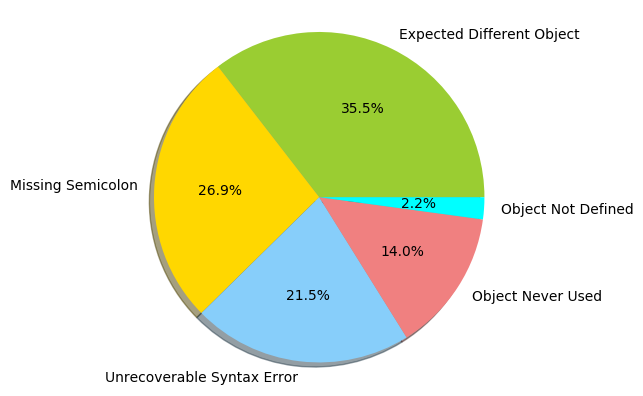
\includegraphics[width=\textwidth, keepaspectratio]{images/MCE2-npmchar.png}
\end{figure}

\begin{figure}
	\caption{Συνηθέστερο λάθος των αρχείων του \en{labeled-char-rnn}}
	\label{MCE1-npmlabeled}
	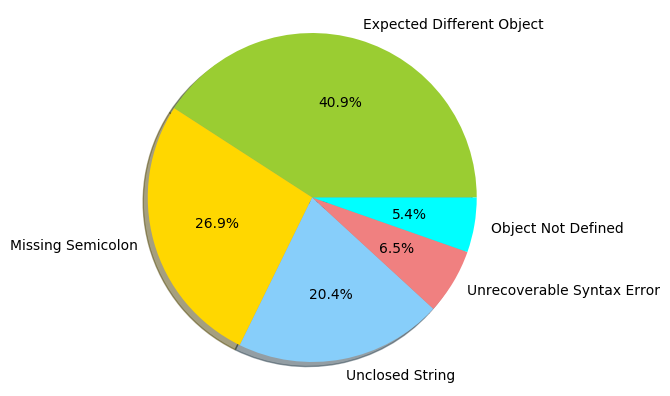
\includegraphics[width=\textwidth, keepaspectratio]{images/MCE-npmlabeled.png}
\end{figure}

\begin{figure}
	\caption{Δεύτερο συνηθέστερο λάθος των αρχείων του \en{labeled-char-rnn}}
	\label{MCE2-npmlabeled}
	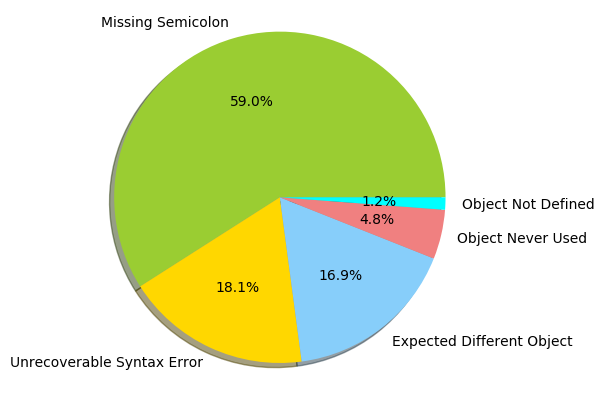
\includegraphics[width=\textwidth, keepaspectratio]{images/MCE2-npmlabeled.png}
\end{figure}

\pagebreak 

\subsection{\en{Top 100 Github Javascript Projects} Παραγώμενος κώδικας με αλλοιωμένη δειγματοληψία}

Η δυνατότητα παραγωγής κώδικα οφείλεται, εν μέρει, στην προσθήκη της δειγματοληψίας της εξόδου του συστήματος μας. Με σκοπό τη διερεύνηση της λειτουργίας των δύο μοντέλων, θα αλλοιώσουμε την κατανομή πιθανότητας που προτείνει το μοντέλο, ώστε να είναι πιο σίγουρο για τις προβλέψεις του. Χρησιμοποιούμε την συνάρτηση \en{Softmax Temperature} και επιλεγμένη τιμή για τη θερμοκρασία  0.85. Επιλέγουμε τα μοντέλα που εκπαιδεύτηκαν στο \en{Top 100 Github js dataset} και τον ίδιο κώδικα αρχικοποίησης που χρησιμοποίησαμε παραπάνω. Οι κώδικες 5.7, 5.8 περιέχουν αρχεία που παρήχθησαν από τα 2 μοντέλα. Στο κόστος της ποικιλίας του παραγώμενου κώδικα, τα μοντέλα κάνουν πιο <<συνηθισμένες>> επιλογές.   

\selectlanguage{english}
\lstinputlisting[language=JavaScript, caption={\tg{Δείγμα κώδικα απο το }\en{char-rnn}\tg{ με αλλοιωμένη δειγματοληψία}}]{code/temp-char.js}
\selectlanguage{greek}

\pagebreak

\selectlanguage{english}
\lstinputlisting[language=JavaScript, caption={\tg{Δείγμα κώδικα απο το }\en{labeled-char-rnn}\tg{ με αλλοιωμένη δειγματοληψία}}]{code/temp-labeled-char.js}
\selectlanguage{greek}

Στις εικόνες \ref{static-temp-char} - \ref{MCE2-temp-labeled} παρατίθενται τα αποτελέσματα της ανάλυσης.
Το μέσο μήκος των παραγώμενων αρχείων ανεβαίνει σημαντικά σε σχέση με τις προηγούμενες προσεγγίσεις (218 - 132 γραμμες).
Όπως και στα προηγούμενα αποτελέσματα, το μοντέλο \en{labeled-char-rnn} κλείνει με μεγαλύτερη συνέπεια τα αρχεία του, αλλά τα παραγώμενα αρχεία ολοκληρώνουν σε μικρότερο ποσοστό τον συντακτικό έλεγχο επιτυχημένα.
Ενδιαφέρουσα είναι η εμφάνιση του λάθους \en{'Object Already Defined'} στα πιο συνηθισμένα λάθη.
Πράγματι, τα αρχεία που παράγονται απο τα μοντέλα, τα οποία έχουν μεγαλύτερη πεποίθηση για τις προβλέψεις τους, τείνουν να επαναλαμβάνουν διάφορες δομές και λάθη.

\begin{figure}
	\caption{Στατική ανάλυση κώδικα για τα αποτελέσματα του \en{char-rnn} μοντέλου}
	\label{static-temp-char}
	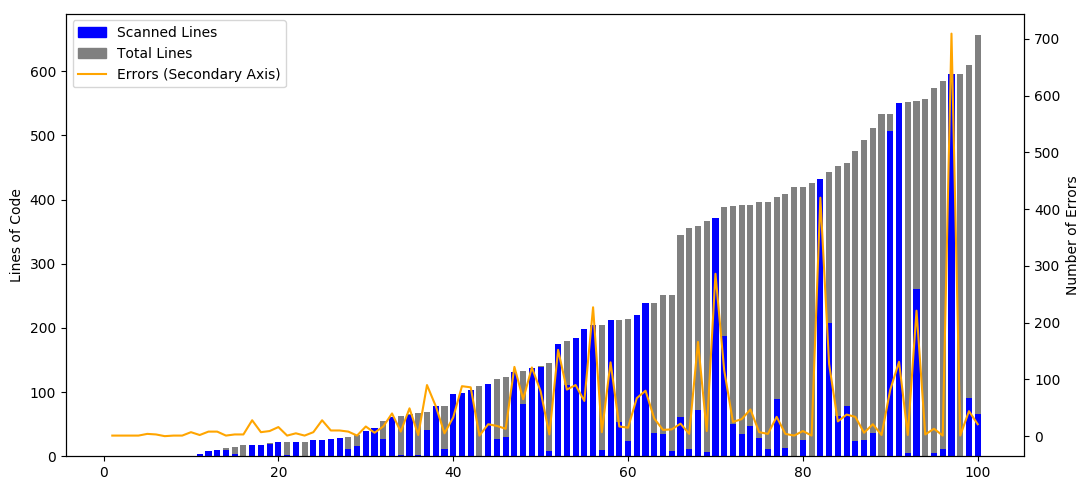
\includegraphics[width=\textwidth, keepaspectratio]{images/temp-char.png}
\end{figure}

\begin{figure}
	\caption{Στατική ανάλυση κώδικα για τα αποτελέσματα του \en{labeled-char-rnn} μοντέλου}
	\label{static-temp-labeled}
	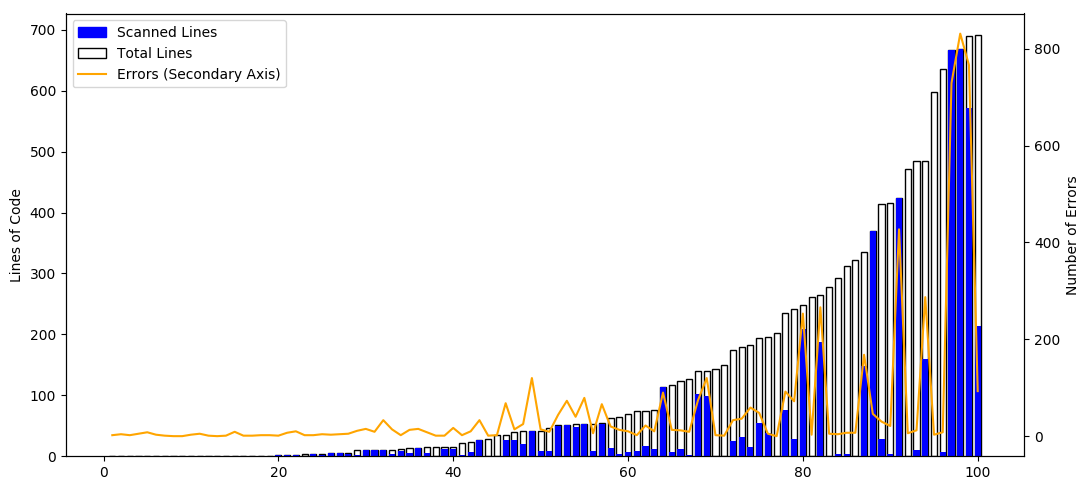
\includegraphics[width=\textwidth, keepaspectratio]{images/temp-labeled.png}
\end{figure}

\begin{figure}
	\caption{Συνηθέστερο λάθος των αρχείων του \en{char-rnn}}
	\label{MCE-temp-char}
	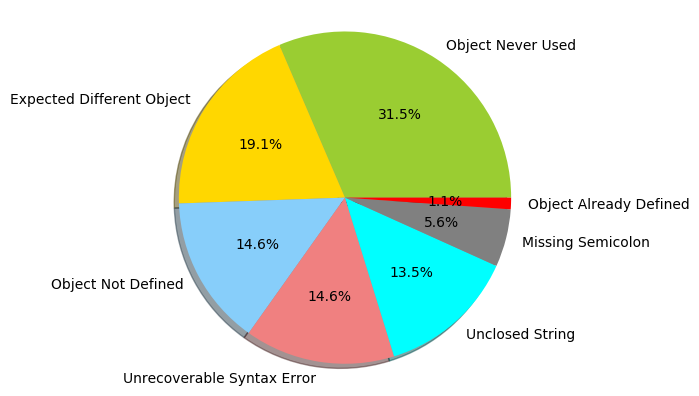
\includegraphics[width=\textwidth, keepaspectratio]{images/MCE-temp-char.png}
\end{figure}

\begin{figure}
	\caption{Δεύτερο συνηθέστερο λάθος των αρχείων του \en{char-rnn}}
	\label{MCE2-temp-char}
	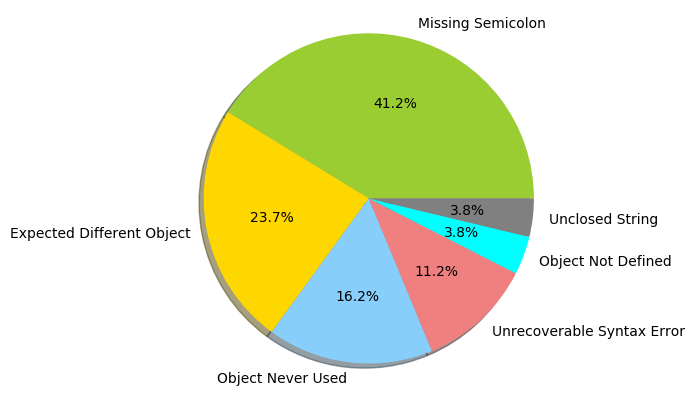
\includegraphics[width=\textwidth, keepaspectratio]{images/MCE2-temp-char.png}
\end{figure}

\begin{figure}
	\caption{Συνηθέστερο λάθος των αρχείων του \en{labeled-char-rnn}}
	\label{MCE2-temp-labeled}
	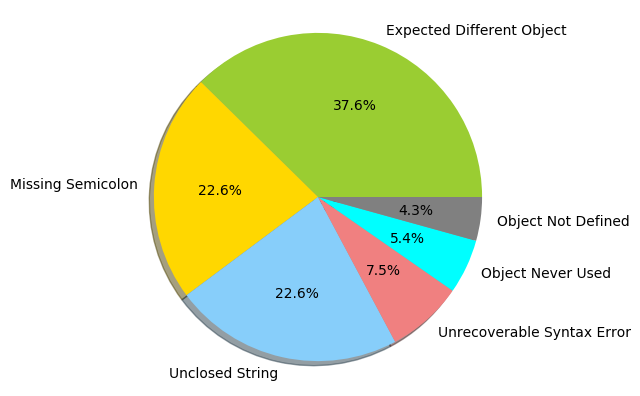
\includegraphics[width=\textwidth, keepaspectratio]{images/MCE-temp-labeled.png}
\end{figure}

\begin{figure}
	\caption{Δεύτερο συνηθέστερο λάθος των αρχείων του \en{labeled-char-rnn}}
	\label{MCE2-temp-labeled}
	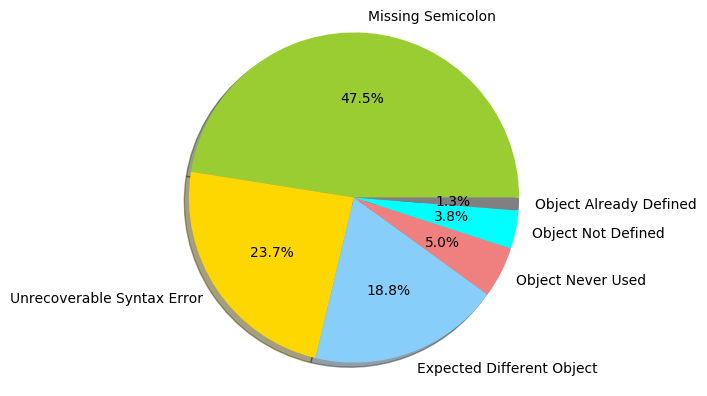
\includegraphics[width=\textwidth, keepaspectratio]{images/MCE2-temp-labeled.png}
\end{figure}

\subsection{Σχόλια περί σύγκρισης}

Τα αποτελέσματα της παραγωγής κώδικα που δεν είναι πραγματικά λειτουργικός είναι δύσκολο να ποσοτικοποιηθούν. Η εγγενής δυσκολία ερμήνευσης της εκμάθησης των νευρωνικών δικτύων, δυσκολεύει περαιτέρω την προσπάθεια αυτή. Με σκοπό την αποσαφήνιση των αποτελεσμάτων, δημιουργούμε μία απλή μετρική ώστε να συγκρίνουμε τα 6 μοντέλα που δοκιμάστηκαν.

\begin{equation}
M = Mean\ \#\ Errors / (Mean\ \#\ Lines * Mean\ Syntax\ Analysis\ Completion\ \%)
\end{equation}

\begin{table}[!h]
\centering
\caption{Τιμές της Μετρικής $M$ για τα μοντέλα που δοκιμάστηκαν}
\begin{tabularx}{\textwidth}{|X|X|X|}
\hline
                    & \en{char-rnn} & \en{labeled-char-rnn} \\
\hline
\en{Github}       & 0.61             & 0.86                     \\
\hline
\en{NPM}       & 0.64             & 0.77                  \\
\hline
\en{Github Temperature}       & 0.38             & 0.52                  \\
\hline
\end{tabularx}
\label{Mtable}
\end{table}

Από τον πίνακα \ref{Mtable} μπορούμε να εξάγουμε 2 σημαντικά παρατηρήσεις (Μικρότερες τιμές του $M$ είναι προτιμότερες).
Αρχικά, το μοντέλο \en{labeled-char-rnn} έχει σταθερά χειρότερες επιδόσεις στην παραγωγή ποιοτικού κώδικα, παρόλο που έχει στη διάθεση του παραπάνω πληροφορία για τον κώδικα και μάλιστα σημαντική. Αυτό οφείλεται εν μέρει στην ταυτόχρονη στοχαστική επιλογή χαρακτήρα και είδους του, που μπορεί να επινοεί συνδυασμούς που δεν έχει ξαναδεί. Έπειτα η στοχαστικότητα που εισάγεται για την παραγωγή κώδικα δυσκολεύει γενικότερα τα μοντέλα να γράψουν ορθά προγράμματα, για αυτό και όταν επιβάλλουμε στα συστήματα να εμπιστεύονται τις προβλέψεις τους, παίρνουμε καλύτερες τιμές για τη μετρική $M$.